% System architecture diagram (TikZ). Included from chapters/03_methodology.tex
\usetikzlibrary{positioning,arrows.meta,shapes,fit,backgrounds}
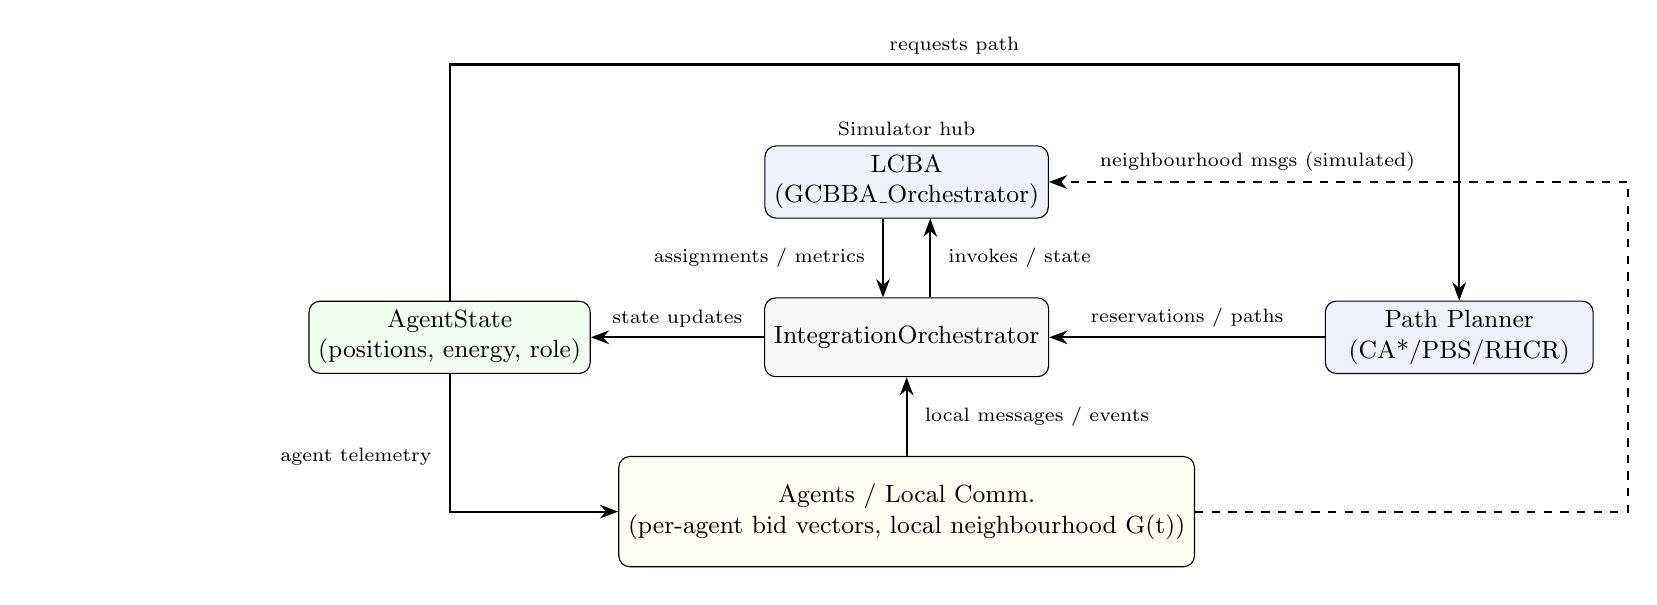
\begin{tikzpicture}[node distance=20mm, >=Stealth, every node/.style={font=\small}]
  % Styles
  \tikzset{
    comp/.style={draw, rounded corners, minimum width=36mm, minimum height=10mm, align=center, fill=gray!6},
    module/.style={draw, rounded corners, minimum width=34mm, minimum height=8mm, align=center, fill=blue!6},
    data/.style={draw, rounded corners, minimum width=30mm, minimum height=7mm, align=center, fill=green!6},
    arrow/.style={->, thick}
  }

  % Nodes
  \node[comp] (io) {IntegrationOrchestrator};
  \node[module, above=10mm of io] (gcbba) {LCBA \\ (GCBBA\_Orchestrator)};
  \node[module, right=35mm of io] (planner) {Path Planner \\ (CA*/PBS/RHCR)};
  \node[data, left=22mm of io] (agentstate) {AgentState \\ (positions, energy, role)};
  \node[draw, rounded corners, below=10mm of io, minimum width=70mm, minimum height=14mm, align=center, fill=yellow!6] (agents) {Agents / Local Comm. \\ (per-agent bid vectors, local neighbourhood G(t))};

  % Annotation
  \node[anchor=south, font=\scriptsize] at (gcbba.north) {Simulator hub};

  % Arrows: gcbba <-> io (x-shifted to avoid overlap)
  \draw[arrow] ([xshift=3mm]io.north) -- ([xshift=3mm]gcbba.south)
      node[midway, right=1mm, font=\scriptsize] {invokes / state};
  \draw[arrow] ([xshift=-3mm]gcbba.south) -- ([xshift=-3mm]io.north)
      node[midway, left=1mm, font=\scriptsize] {assignments / metrics};

  % agentstate -> planner: route above gcbba to avoid crossing io
  \draw[arrow] (agentstate.north) -- ++(0,30mm) -| (planner.north)
      node[pos=0.25, above, font=\scriptsize] {requests path};

  % planner -> io
  \draw[arrow] (planner.west) -- (io.east)
      node[midway, above, font=\scriptsize] {reservations / paths};

  % io -> agentstate
  \draw[arrow] (io.west) -- (agentstate.east) node[midway, above, font=\scriptsize] {state updates};

  % agentstate -> agents (right-angled: down then right into agents.west)
  \draw[arrow] (agentstate.south) |- (agents.west)
      node[pos=0.3, left=1mm, font=\scriptsize] {agent telemetry};

  % agents -> io
  \draw[arrow] (agents.north) -- (io.south)
      node[midway, right=1mm, font=\scriptsize] {local messages / events};

  % agents -> gcbba (dashed, neighbourhood msgs): route right of planner, then up, then left
  \draw[arrow, dashed] (agents.east) -- ++(55mm,0) |- (gcbba.east)
      node[pos=0.82, above, font=\scriptsize] {neighbourhood msgs (simulated)};

  % Phantom path on left to balance bounding box (makes centering symmetric around io)
  \path ([xshift=-75mm]agents.west);

  % Background fit (visual grouping)
  \begin{scope}[on background layer]
    \node[fit=(gcbba)(planner)(agentstate)(io)(agents), draw=none] {};
  \end{scope}
\end{tikzpicture}
